
\documentclass{article}

\usepackage{arxiv}
\usepackage{graphicx}

\usepackage[utf8]{inputenc} % allow utf-8 input
\usepackage[T1]{fontenc} % use 8-bit T1 fonts
\usepackage{hyperref} % hyperlinks
\usepackage{url} % simple URL typesetting
\usepackage{booktabs} % professional-quality tables
\usepackage{amsfonts} % blackboard math symbols
\usepackage{nicefrac} % compact symbols for 1/2, etc.
\usepackage{microtype} % microtypography
\usepackage{lipsum}
\usepackage{float}


\title{Review of current ultrasound hardware considerations, designs, and processing opportunities}





\author{
 Luc Jonveaux\thanks{Lead of the un0rick.cc project } \\
 Open-source hobbyist \\
 Milly le Meugon, FR\\
 \texttt{kelu124@gmail.com} \\
 \And
 Carla Schloh \\
 Fraunhofer MEVIS\\
 Institute for Digital Medicine\\
 Bremen, DE\\
 \texttt{ carla.schloh@mevis.fraunhofer.de} \\
\And
 William Meng \\
Columbia University \\
 New York, US\\
 \texttt{ wlm2117@columbia.edu} \\
 %% examples of more authors
 \And
 Jorge Arija \\
MicroComp \\
 Bilbao, ES\\
 \texttt{ jarija@microcomp.es} \\
   \And
 Jean Rintoul \\
Mindseye Biomedical \\
 London, UK\\
 \texttt{ jean@mindseyebiomedical.com} \\
 }


\begin{document}
\maketitle

\begin{abstract}

Ultrasound imaging is one of the most widely used tools for non-destructive testing and non-invasive diagnostic medicine.
Since its beginnings in the 1970s, ultrasound remains an active field of research,
with innovations such as new sensors, signal processing, and hardware development.

However, within the realm of open-source methodology, the field remains under-served in terms of experimental hardware.
An open, highly flexible and cost-efficient platform is still needed for many medical and biological applications, to support the efforts of the researchers, makers and device developers and accelerate ultrasound research and development.

In the pursuit of designing a single-element pulse-echo device, it is necessary to map the current state of research in the field. Hereby, questions such as how the ultrasound hardware is used, which components the hardware architecture of an ultrasound device incorporates and what specifications are required, arise. 

The aim of this paper is to identify relevant literature to consider when designing a simple open-source single-channel ultrasound device and make this body of knowledge accessible to the maker and hobbyist designer. This includes usage considerations, hardware, embedded code, and software considerations.
\end{abstract}


% keywords can be removed
\keywords{ultrasound \and hardware \and open-source \and frugal device \and imaging \and single-element \and modular design}

% this table is to be removed before submission
%\tableofcontents

\newpage


\section{Context}

\subsection{Why Ultrasound is Interesting}

Ultrasound imaging was initially developed by Langevin for underwater sonar uses, based on the piezoelectric effect discovered by the Curie brothers. Moreover, ultrasound has been a developing field for medical imaging and non-destructive testing and exploration (NDT/NDE) since the 1950s, such as with the Sonovisor device \cite{zeiss_sonovisor_1962}. Although ultrasound is a mature technology, it remains an active field of study, and  technologies yet to be further explored, such as compressed sensing \cite{kruizinga_compressive_2017,liebgott_compressive_2012} have the potential to revolutionize low-cost ultrasound imaging.
Therefore, it makes sense to build an affordable and extensible platform for ultrasound research that leverages advances in low-cost computing in order to offload functions which previously required dedicated hardware.

Ultrasound imaging has numerous advantages over other widely-used imaging modalities such as Computer Tomography (CT) or Magnet Resonance Tomography (MRI), especially because it is deemed safe and affordable. Due to these characteristics \cite{kurjak_use_1986}, it has become an important tool in medical care. The World Health Organisation \cite{who_future_1985} recognises and stresses the advantages of using ultrasound in medically under-served regions such as Low and Middle Income Countries where other technology is simply not affordable or the infrastructure non-existent. High-end systems, as used in clinics, are mounted on a trolley to be moved to the patient’s bedside). Smaller systems referred to as “Hand-Held Devices” (HHD), which have the dimensions of a laptop computer or are even smartphone-sized and are subject to recent research in the field of medical ultrasound imaging. HHD hold the potential to become a “game-changing” technology\cite{kjeken_systematic_2011}. At the same time, the cost of an ultrasound machine is relatively low, compared to other modalities.

\subsection{Ultrasound Imaging Modes}

In general, and except in Doppler imaging, ultrasound imaging is based on the "pulse-echo" principle, based on the dual receiver-transmitter function of a piezoelectric transducer. These modes can be listed as :

\textbf{\textit{A-Mode}}, or Amplitude Mode, is used to display the direct amplitude of echoes received as a function of time, and creates one-dimensional images.

\textbf{\textit{B-Mode}} is the display of a 2D image that is the most common form of ultrasound imaging. It displays the recorded signals' envelope typically in grey-value representation on a 2D map where every value is assigned a shade of grey. The higher the echoes intensity, the brighter the reflection interface is showing in the reconstructed image: this is the widely known unborn baby sonogram.

Other modes, such as M-Mode and C-Mode, combine or extend the aforementioned modes.

\textbf{\textit{Tomography}}: though less common than the previously cited usages, ultrasound can be used in tomography for soft tissues \cite{zhang_design_2015,duric_detection_2007,wen_design_2019,ashfaq_new_2004} where a transducer or array of transducers is used to measure acoustic impedance at different angles, and an image is reconstructed using back-projection or related finite element techniques. The same acoustic impedance methods used in tomography are also used to recreate images with high temporal and spatial resolution in recent works using plane wave acoustic imaging\cite{Rabut2019}, as well as translational work from geophysics in acoustic full-wave inversion\cite{Warner2013}. Witte and Tanter have also pioneered acoustoelectric imaging systems which are able to combine the acoustic image with a current source density image, pointing to promising novel applications in electrophysiology\cite{Xi2009,Qin2017}. New computing techniques have also opened doors to better imaging \cite{guasch_full-waveform_2020,rymarczyk_logistic_2019}. 

%% cite the zhang_design_2015 references for tomography / waag et duric 2 articles @ljo

\subsection{Existing Applications}

\textbf{\textit{Overall imaging}}: Although it is relatively simple and does not enable 2D imaging, A-mode enables 
measurements for examinations such as para-nasal sinuses, trans-skull fluid detection, sinus pathology, skeletal muscle detection in the wrist extension \cite{noauthor_wrist_nodate}, measurement of the carotid artery lumen diameter \cite{li_new_2014,hu_design_2011,zhang_multi-channel_2017,shomaji_early_2019}, bone porosity \cite{wahab_design_2016,fontes-pereira_monitoring_2018,grasel_characterization_2017} or ophthalmology assessments \cite{carotenuto_very_2004}. \textbf{\textit{Vascular measurements}} presents a combination of ultrasound imaging and photoplethysmography are used to measure the diameter and the blood pulse speed traveling through the radial artery \cite{worthing_using_2016}, which then can be used to track changes in blood pressure at various points on the human body. Artery stiffness measurements \cite{joseph_technical_2015,joseph_artsenstouch_2015,seo_non-invasive_2018}. Other \textbf{\textit{body monitoring}} uses can include monitoring bone density \cite{wahab_design_2016,fontes-pereira_monitoring_2018}, muscle assessment \cite{brausch_towards_2019} and quantifying neuromuscular disease progression \cite{zhang_design_2015}, both using A-mode and B-mode imaging, or even tissue assessment \cite{keyes_electrical_2017}. \textbf{\textit{Body composition assessment}} is another application of A-mode imaging \cite{wagner_validity_2016,martins_-scan_2017}. The measurement of \textbf{\textit{bladder volumes}} is also a standard use \cite{kuru_feasibility_2019}, and has become a medical tool. Another use can be providing \textbf{\textit{biofeedback}}: it has been shown that ultrasound also enables the tracking of fingers movement \cite{sikdar_novel_2014}, or , follow-up of biofeedback in stroke reeducation \cite{sosnowska_training_2019} or to \textbf{\textit{tracking body movements}} : the tracking of OSA (Obstructive Sleep Apnea) \cite{weng_fpga-based_2015}, but also of breathing patterns \cite{shahshahani_ultrasound_2018} or heart muscle behavior \cite{nguyen_estimating_2019}.

Other interesting uses include the development of \textbf{\textit{ultrasound Capsules}}, typically a swallowable device, enabling endoscopy imaging using high frequency ultrasound, fitting all the hardware in a 10mm diameter by 30 mm long capsule \cite{cox_ultrasound_2017,wang_development_2017}. Capsules promise further development and their architecture can be a source of inspiration \cite{lee_towards_2014,memon_capsule_2016,lay_progress_2016,lay_-vivo_2018}. \textbf{\textit{ Wearable devices}} are also gaining momentum, due to the miniaturisation trend of components and sensors \cite{basak_wearable_2013}. This is seen also for \textbf{\textit{neuromodulation}} \cite{pashaei_flexible_2020}, where, interestingly, ultrasound can be used to both power the devices and communicate with them \cite{johnson_stimdust_2018,seo_wireless_2016,santagati_design_2020}.

Ultrasound can also be used for \textbf{\textit{nondestructive testing (NDT)}} or nondestructive examination (NDE)  \cite{duncan_real-time_1990}, for quality or integrity control of mechanical elements. \cite{fritsch_full_nodate} presents a very interesting design for single element FPGA-based NDE design, migrating traditionally analog functions, like filtering and envelope extraction to the digital domain developed by others  \cite{triger_modular_2008,shrisha_fpga_2018,rodriguez-olivares_improvement_2018}. 

\subsection{Why commercial medical ultrasound is not easily accessible}

Accessible ultrasound technologies remain somehow limited to researchers. Commercial medical systems are expensive, bulky, not accessible to non-medical staff, and mostly not adapted for research. Some pieces of equipment are adapted for research: they are relatively more flexible, but focus on designs for complex sensors, while keeping costs high. The system architecture of a modern ultrasound system is quite complex and typically out of scope for a maker. The high cost of the commercially-available ultrasound equipment arises from a complex system architecture, expensive sensors, and costly certification process necessary for a product to be put on the market. However, cost is not the main criteria for researchers \cite{chagas_haves_2018}. Furthermore, software and hardware are issued under patents and licenses, preventing researchers from adapting these tools to specific requirements.

Older equipment is available at less cost, but with drastically reduced capabilities. In contrast, ultrasound equipment from the 1970s-80s designed for single element systems, were significantly less complex. To understand and appreciate electronics and mechanical designs, old mechanical probes can easily be procured : it is possible to do with veterinary single-element designs found today. Other designs were proposed by researchers over the two last decades, which will be reviewed below. 

\subsection{Open-source medical hardware}

Open-hardware lowers barriers \cite{pandey_open_2019} in product research: having a full design under an open-source license provides the key to all to contribute and improve a design. This in turns allows a possible rapid spread of the design, customisation for specific uses, and ad-hoc modification. A design being open means that a higher number of contributors can help inspect and improve it. Open source hardware can be a disruptive tool on the medical device market. Shorter development cycles, even for hardware, with open source permits quick iterations over a product, for which economic impacts can be significant \cite{pearce_quantifying_2015,pearce_return_2016,moritz_economic_2019,winter_open_2019}.

As medical hardware and devices, it is essential to ensure that the tools will have the functions they are designed to do: quality and medical certification are key. As such, certification of open-hardware designs is a challenge that needs to be tackled, starting for example from a CE marking perspective. Alternatively, it has been proposed to fund certification by crowd-funding approaches \cite{de_maria_safe_2018}. Of all the medical devices donated to the developing world, 70–90 percent do not function as intended and 20 percent are not used because of poor documentation and training on usage of the devices, according to the WHO \cite{niezen_open-source_2016}. Since their hardware and software architecture are not public knowledge, it is impossible for users to access and repair it. Using open-source products, this problem could be avoided and quite contrarily, support could be available online on how to repair the systems \cite{gibney_open-hardware_2016}.

\newpage
\section{Designing the system architecture}

The following paragraphs give an overview over the field of open-source ultrasound hardware available and existing hardware architectures, based on an earlier similar review \cite{jonveaux_arduino-like_2017}.
Other works describe more complex designs \cite{roman_open-source_2019}, or with sources yet to be completed \cite{enwia_open-source_2019,echopen_echopen_nodate}.


\subsection{Sourcing information}

Apart from the projects described in this paper that aim at developing open-source ultrasound hardware \cite{roman_open-source_2019,luc_jonveaux_un0rick_2019}, several sources of information can be used to feed the design stage.  

For example, the teardown of medical devices available online releases information about the state of the art in terms of hardware architecture. This is mitigated by a low number of occurrence's, as this activity requires both particular skills and interest in dismantling expensive equipment. 

Alternatively, pieces of refurbished equipment, presenting technologies from the 80's and 90's, such as mechanical probes, can provide sensors and ideas from a design perspective, at an affordable cost.  

Chip makers, can be considered actors in knowledge and know-how diffusion \cite{brunner_how_2002,xu_challenges_2010}, being a major producer of concept and design notes. Chip makers also provide guidance on designs \cite{ching_chu_designing_nodate}, but the integration of these components proves to be challenging. For example, datasheets may still be incomplete or erroneous. To support the use of these circuits, chip makers also have proposed evaluation kits - but those may be overly complex for a simple hobbyist, and somehow expensive.

Equipment suppliers, such as Verasonics \cite{peyton_front-end_2017,wall_high-speed_2010,george_portable_2018,hager_lightprobe:_2019,pashaei_flexible_2020,kang_new_2017,boni_ultrasound_2018,wang_high-resolution_2019,hager_ultralight:_2017,peyton_comparison_2018,assef_initial_2016} or Lecoeur-electronics \cite{lecoeur_bluetooth_nodate,tortoli_ula-op:_2009,zhang_toward_2018,al-aufi_thin_2019}, Ultratek \cite{veenstra_generating_nodate,perez-sanchez_numerical_2020,chen_ultrasound_2016,wang_preliminary_2019}, Optel \cite{veenstra_generating_nodate,scholle_pulse_2018,ratajski_application_2017,nowak_evaluation_2020}, Eurosonic \cite{vadalma_smartphone_2020}, Biosono \cite{biosono_sonolab_nodate} or even the Fraunhofer institute \cite{zimmermann_highly_2019,zimmermann_miniaturized_2018,zimmermann_high_2018} provide researchers with similar equipment, making it possible to better understand the required functionalities.
% luc @tomerge :  
%-optel (2.1 opbox the best)
%-lecoeur electronique (US-box, Us-smart)
%-mistras Eurosonic (UTC110-4 encoders, USB-8M)
%-us Ultratek (USB-UT350, USB-UT350T)  

\subsection{Functional blocks}

The functions required in an ultrasound system are relatively standard, and  are depicted in figure \ref{fig:BlockDiagramme}.

\begin{figure}[H]
 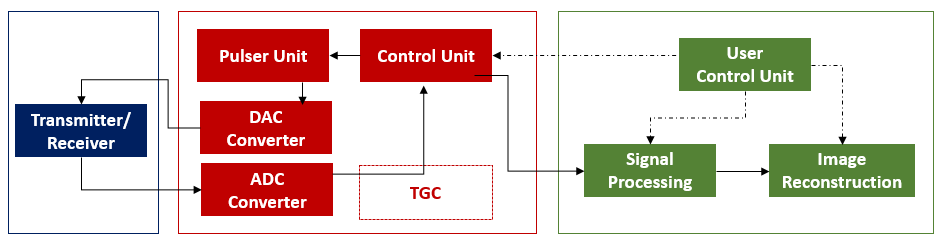
\includegraphics[width=\linewidth]{images/Blockdiagramme.PNG}
 \caption{Block Diagram of Single-Element Ultrasound System, showing the functions needed for a simple ultrasound device}
 \label{fig:BlockDiagramme}
\end{figure}
These blocks are used to create the pulse-echo pattern that ultimately creates an ultrasound image.

\begin{figure}[H]
 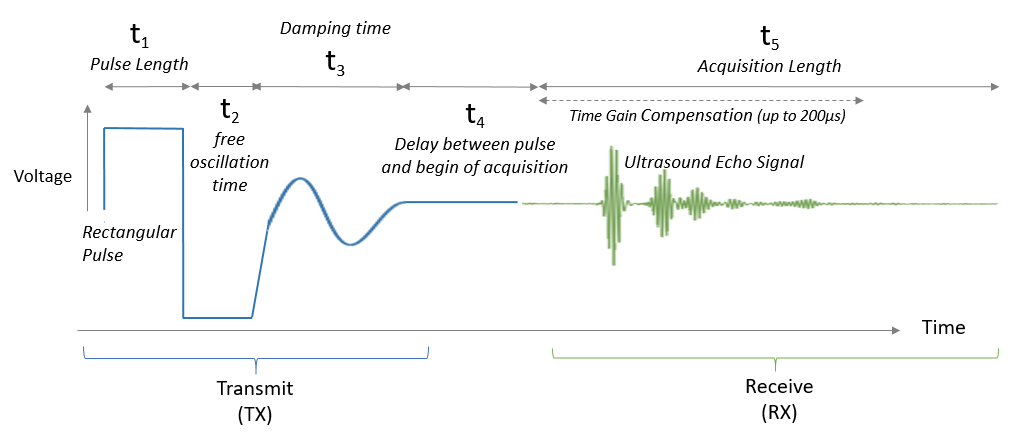
\includegraphics[width=\linewidth]{images/PulseTrain.PNG}
 \caption{Pulse Train of a pulse echo device. Transmit (blue) and Receive (green) path}
 \label{fig:PulseTrain}
\end{figure}




\subsection{Earlier works on a simple hardware architecture for ultrasound systems}

The first research setup appears to date back to 1993 \cite{jensen_deconvolution_1993}, where a Bruel \& Kjaer, BK Type 1846 was modified to accept research equipment.
From then, apart from designing medical probes, several groups of researchers have worked since the early 2000s to design research-friendly equipment. Most of these designs are for multi-channel \cite{boni_ula-op_2016,boni_reconfigurable_2012,boni_ultrasound_2018,qiu_flexible_2012,levesque_architecture_2011}, but other consider single element designs, such as \cite{carotenuto_fast_2005}, or \cite{richard_low-cost_2008}. An interesting modular design was proposed by \cite{wall_high-speed_2010} using a motherboard connected. More recently, \cite{taylor_development_2017} also used a beagle bone device. \cite{jonveaux_arduino-like_2017} proposed an Arduino-like approach to functional blocks, balanced by SNR and cost impacts, which possibly inspired further designs \cite{golabek_construction_2019}.

\subsection{State-of-the-Art and review of the ultrasound hardware designs}

\subsubsection{General state of the art review}

A review of the literature with respect to ultrasound system designs was summarized in the table below, based on a systematic review of components used.

% Please add the following required packages to your document preamble:
% \usepackage{booktabs}
 
\begin{table}[H]
\centering
\begin{tabular}{l|c|c|c|c|c|c}
\textbf{Reference}                               & \textbf{Elements} & \textbf{Voltage} & \textbf{Msps} & \textbf{Res} & \textbf{AFE-TGC}    & \textbf{Year}   \\ \hline
\cite{ahn_smartphone-based_2015}    & 16          & 70V     & 40   & 10   & AFE5808 & 2015 \\
\cite{assef_compact_2014}      & 128         & 100 Vpp & 50   & 12   & AFE5805 & 2014 \\
\cite{assef_design_2012}       & 128         & 100 Vpp & 50   & 12   & AFE5805 & 2012 \\
\cite{assef_flexible_2015}          & NA          & 100 Vpp & 40   & 12   & AFE5805 & 2015\\
\cite{batbayar_hardware_2018}     & 4x32        & NA      & 80   & 10   & NA      & 2018 \\
\cite{bharath_compact_2018}  & 8           & 105V    & 50   & 16   & AFE5809 & 2018 \\
\cite{bharath_novel_2016}     & 8           & +-50V   & 40   & 12   & AFE5808 & 2016 \\
\cite{bharath_portable_2015}      & NA          & NA      & NA   &      & NA      & 2015 \\
\cite{chang-hong_hu_design_2008}   & 1           & 15V     & 120  & 12   &         & 2008 \\
\cite{chatar_analysis_2016}        & 16          & NA      & 150  & 14   & NA      & 2016 \\
\cite{cheung_multi-channel_2012} & 128         & NA      & 80   & 10   & AD9272  & 2012 \\
\cite{dusa_low_2014}             & 8           & 100 Vpp & 65   & 12   & AFE5809 & 2014 \\
\cite{fritsch_full_nodate}          & 1           & 50-400V & 80   &      & NA      & NA \\
\cite{govindan_reconfigurable_2015} & 8           & NA      & 250  & 8    & VCA8500 & 2015 \\
\cite{hager_ultralight:_2017} & 64          & 100Vpp  & 32,5 & 12   & AFE5851 & 2017 \\
\cite{hewener_highly_2012}      & 128         & +-75V   & 80   &      & AD9273  & 2012 \\
 \cite{ibrahim_towards_2018}     & 64          & 12 V    & 20   & 12   & NA      & 2018 \\
 \cite{jonveaux_arduino-like_2017} & Single      & 100Vpp  & 22   & 9    & AD8331  & 2018 \\
 \cite{kim_smart-phone_2017}       & 128 (32 ch) & +-80 V  & 50   & 12   & NA      & 2017 \\
\cite{kruizinga_compressive_2017}  & Single      & 100 Vpp & 200  & 12   & NA      & 2017 \\
\cite{kushi_ultrasonic_2017}     & Single      & NA      & 100  & 14   & NA      & 2017 \\
\cite{lee_new_2014}             & 16          & NA      & 40   &      & AFE5808 & 2014 \\
\cite{li_new_2014}         & Single      & 80 V    & 40   & 12   & AD9276  & 2014 \\
\cite{matera_smart_2018}       & 8           & 6V      & 75   & 14   & AFE5809 & 2018 \\
\cite{nguyen_estimating_2019}    & 2           & 18V     & 40   & 10   &         & 2019 \\
\cite{pashaei_flexible_2020}      & 8           & 10V     & 80   & 12   & AD9276  & 2020 \\
 \cite{peyton_comparison_2018}     & 32          & NA      & 20   &      & Custom  & 2018 \\
\cite{qiu_delayed-excitation_2018} & Single      & +48V    & 160  &      & AD8331  & 2018 \\
\cite{qiu_ultrasound_2020}         & 1           & 60V     & 250  & 12   & TC6320  & 2020 \\
\cite{ricci_programmable_2006}   & 1           & 100 V   & 64   & 14   & MAX4107 & 2006 \\
\cite{roman_open-source_2018}   & 64          & +-50V   & 80   & 12   & AD9276  & 2018 \\
 \cite{vasudevan_programmable_2014} & Single      & 100 Vpp & 250  & 12   & VCA8500 & 2014 \\
\cite{wall_high-speed_2010}        & NA          & 12 V    & 65   &      & NA      & 2010 \\
\cite{weng_fpga-based_2015}      & 16          & 100V    & 150  & 10   & Max2077 & 2015 \\
\cite{zhang_high_2019}            & 64          & 100V    & 80   & 14   &         & 2019 \\
\cite{zhang_multi-channel_2017}     & 8           & 70V     & 250  & 16   & QT1138  & 2017    

\end{tabular} 
\caption{Review of ultrasound hardware designs, detailing speed of acquisitions (Msps), Resolution (Res.) and possibly the other supporting devices}
\label{tab:benchmarklite}
\end{table}


\subsubsection{AFE}

It appears that most research designs use all-integrated Analog Front-End (AFE), which allow for a simpler design, at the cost of integrating several functions into NDA-covered chips, and which can make a design more expensive and less open. Different chips families were identified during this state-of-the-art review. The \emph{AD927X} have usually 8 channels, with a 12-bit ADC from 10 MSPS to 80 MSPS, with full LNA, VGA, and AAF, widely used \cite{hewener_highly_2012,alqasemi_fpga-based_2012,di_ianni_system-level_2016,raj_programmable_2018,raj_microcontroller_2017,cheung_multi-channel_2012,alqasemi_fpga-based_2012,batbayar_hardware_2018,raj_8051_2016,li_new_2014,enwia_open-source_2019,techavipoo_ultrasound_2012,pashaei_flexible_2020,shomaji_early_2019,roman_open-source_2018}. More design considerations were researched by \cite{di_ianni_system-level_2016}.
The \emph{AFE58XX} familly has 8 to 32 channels AFEs, from 50-65MSPS, with LNA, VCAT, PGA, LPF, ADC, and possibly CW Mixer \cite{assef_flexible_2015,assef_design_2012,assef_compact_2014,assef_initial_2016,bharath_fpga-based_2015,bharath_novel_2016,lee_new_2014,hager_lightprobe:_2017,bharath_compact_2018,kidav_architecture_2019}. Finally, the \emph{MAX2082 and MAX2077} have 8channels including the HV Pulser, TR-Switch, but present no ADC \cite{hewener_mobile_2019,weng_fpga-based_2015}. 

These AFEs all include several channels, which is not needed in a single-element design. However, they may be useful in multi-channel designs in order to improve space and cost efficiency.

\subsubsection{Managing several channels}

Even if not strictly required for single element pulse-echo devices, multiplexers or high-voltage switches can be used to address several transducers from a single transmit and a single receive path. Options can include dedicated systems such as the HV2605, MAX14866 \cite{enwia_open-source_2019,pashaei_flexible_2020}, or HV20220 \cite{li_new_2014}. Those switches can also be integrated at the pulser level \cite{worthing_using_2016,hidayat_determination_2020} or be integrated on the receiving path, for example with a LM96530 \cite{gwirc_desarrollo_2019,vasudevan_programmable_2014,roman_open-source_2018}.

Another option, beamformers, were commonly observed in research setups, mostly based on a LM965XX \cite{gwirc_desarrollo_2019,yu_low-power_2012,roman_open-source_2018,bharath_fpga-based_2015,roman_open-source_2018}.

\subsubsection{Mechanical Sweeping}

When designing a single-element sensor to produce a 2D image, a system allowing to sweep the space to be imaged is required. Several types of actuators were identified in the review. In general, and to minimize hardware costs, a single piezoelectric element, mechanically swept across the target scene, with the corresponding channel acquisition circuit, as successfully initially shown by \cite{saijo_development_nodate}. This principle was used in older mechanical probes (initially more common in intra-cavity probes due to space constraints). Those are based on either continuous rotation (Kretztechnik AR3 4/5B/A, ATL 724A, ... ) of the transducer to allow for plane sweeping, sometimes with multiple transducers to allow for multiple image per rotation, or with mechanical sweeps (Interspec Apogee, Diasonics probes, Kretztechnik AW14/5B/A, HP 21412A, ... ). This sweeping principle has been re used in multiple experimental setups, such as \cite{chang_low-cost_2009}.

For small-animals cardiac imaging, heartbeat and target size  require high fps, above 100 fps, with a spatial resolution of 100um or less. Lei et al. \cite{lei_high-frame_nodate} achieved an interesting 30-50MHz real-time ultrasound single-element system at 130 fps, using a 22 degree arc at 65Hz, the pulse-echo system being controlled by the motor position. Imaging transducers are also relatively smaller, which makes mechanical a solution of choice, when arrays may be too large. This implies however strong positioning control and precision motors, using for example optical encoder and  piezoelectric	motors \cite{carotenuto_very_2004}, allowing for 256 view lines to build a single frame, at a rate of 15 frames per second. Other uses of piezoelectric actuators include the use of bimorphs \cite{bezanson_low-cost_2011}, which can increase the benchmark of 130fps for electromagnetic motors. Still, the weight borne by the actuator has to be limited \cite{brown_low_2013,huang_novel_2015}, a constraint also satisfied by MEMs \cite{choi_versatile_2020}.

On laboratory designs, where real-time is not an issue, XYZ positioning may also be used \cite{svilainis_electronics_2014,wang_high_2019,xu_enabling_2019}, for example using 3D-printed elements \cite{bottenus_feasibility_2016} showed that a three-axis translation stage allowing precise position and orientation control of the transducer. \cite{qiu_programmable_2011} uses a transducer on a linear motor stage to allow 8 mm/s linear imaging scans to be performed, a tool used in other experiments \cite{govindan_reconfigurable_2015,soto-cajiga_fpga-based_2012}.  \cite{heuvel_development_2017} for example uses a motor as the positioning system to sweep its single transducer across the target scene.  \cite{smith_design_2015} also uses a single transducer element and a mechanical actuator - stating that it reaches a compromise as the image quality is reduced but the cost saving is significant (over 95\% cost reduction). In particular, it explores the possibility  to use a lower-noise voice coil motor (VCM) is ideal for maintaining a high signal to noise ratio of the echo data and the accurate positional encoder allows the ultrasound image to be constructed at the end of each scanning cycle.

Alternative displacements methods can be used, for example using accelerometers to determine the angular position of the transducer  \cite{sobhani_portable_2016}, allowing for precise image reconstruction with an Arduino and Raspberry Pi setup \cite{herickhoff_low-cost_2019},also used in ultrasound training simulators \cite{farsoni_low-cost_2017} . Another example is, in the case of skin imaging, to use an optical tracker present on computer mice \cite{zhang_free-hand_2019,poulsen_optical_2005,herickhoff_low-cost_2018}.

\subsubsection{High voltage tools}


A review of the high-voltage components has been done: however, the topic of efficient high voltage sources is not covered in most of the publications, apart from \cite{xiao_design_2013}. High voltage design for ultrasound has been a particular point of interest. The ideal requirements for a good High Voltage design would be to have a small footprint, low consumption, settable level between 0 to 90V, ideally with another source for 0 to -90V, for bipolar pulses, usually for current supply of 25-30mA.  Early designs \cite{brown_low-cost_2002} managed 350V pulses with \$50\, but this is still a challenge today. In addition, few are sharing their designs \cite{tang_computerized_2014}, even considering existing detailed datasheets (including schematics) \cite{granata_designing_2020}, focusing on flyback and SEPIC configurations. Devices such as LM96550 were not considered because of their relative important size. From the open-source literature, first designs came with a RECOM device, expensive, but with a full 0 - 120V range. Then the NMT0572SC, providing 24, 48 and 72V rails, and the LT3494 with a rail up to 39V. Other alternatives were considered , namely the \emph{MAX668} (going from O to 150V), \emph{MAX1856} between -80V and -24V, a \emph{MIC3172} design, using an \emph{HV9150} to reach up to 200V or a \emph{MAX15031} up to 80V. The \emph{DRV8662} family also has been used to provide rails for up to 105V. Clipping devices (MD0100 \cite{li_new_2014,sharma_development_2015}, MMBD4148/MMBD3004 \cite{ching_chu_designing_nodate}) allow to clipping the signal on the receive path to protect it.

Electrical impedance matching \cite{sharma_development_2015} can be used to also improve the level of energy transmitted to the transducer, especially with low-cost VNAs (eg the 40\$ NanoVNA, usable on MHz-range transducers) - interesting developments \cite{garcia-rodriguez_low_2010,wei_design_2020} can be used for improving overall SNR.

\subsubsection{Materials choice}

On most mechanical designs, an acoustic window is needed to seal the scanner head from the external medium, while minimizing signal loss. The first mechanical scanners used water-baths \cite{schueler_fundamentals_1984} as an intermediate between the transducers and the subject. A material regularly used is TPX (polymethylpentene), used for example on an hand-held high frequency ultrasound scanner \cite{erickson_hand-held_2001}, stating a two-way loss due to the acoustic window of approximately 0.02 dB over a frequency range of 32 to 50 MHz. TPX is also used as an acoustic window on a bimorph design \cite{brown_low_2013}, in which the 45MHz element is located inside a 3D printed probe, allowing for scans at 100Hz. Alternatively, \cite{qiu_ultrasound_2020} uses an acoustic window made from polydimethylsiloxane (PDMS) to minimize the reflection and
attenuation during the ultrasound transmission.

Acoustically interesting materials can also be used. For example polyimide \cite{xu_high-frequency_2008,lei_sun_high-frame_2008} can be used in phantoms as well as sealant silicones \cite{lorenzo_experimental_2009} mimicking soft tissues. Agar and gelatin are used on temporary phantoms \cite{vogt_development_2005,chun_ultrasound_2015}, where graphite powder reproduces tissue scattering. Alternatively, for a good device-patient coupling, polyvinyl alcohol or polyurethane, as well as polyvinylidene fluoride (PVDF) can be considered \cite{sikdar_novel_2014}.

3D-printed parts are in general a very useful supplement to finalise a scanner device. Apart from a holder mechanism to house the transducer, it can provide casing and cover to shield the device. It can also provide functional parts , like aberration masks in the case of compressed sensing applications \cite{kruizinga_compressive_2017}.

\subsection{Minimal specifications}

For the sake of understanding the minimal set of specifications for an ultrasound B-mode scanner, considering minimal specs for B-mode imaging \cite{kurjak_use_1986} laid out the basic specifications for a General Purpose Ultrasound Scanner. Moreover, in terms of ADC selection, one can note that producing a quality image of human tissues require at least 50dB of SNR \cite{attarzadeh_low-power_2017}, requiring a minimum of a 9-bit ADC. This in turn can be used to infer minimal specifications for simple ultrasound pulse-echo devices:

\begin{itemize}
\item be able to do B-mode images, translating in have linear- and convex- type scan-heads
\item with a sensor frequency of at least 3.5MHz - extensible to 5MHz. From there an ADC at at least 15MHz with at least 9 to 10 bit resolution would be indicated;
\item Be displayed on a reconstructed 512 x 512 image, on 4 bits.
\item Images should go to a depth of 18cm, meaning 240us of acquisition, in line with a 512 pixel-deep image considering a single-element resolution. 
\item with a viewing angle of 40 degrees or more, which indicates that 128 lines per image should be sufficient.
\item image should be refreshed at 5 to 10fps.
\end{itemize}

A target of 10 fps, leads to 780us between lines (and less than 700ksps), which is in line with the requirements, and manageable by modern buses. 



\newpage
\section{Further hardware signal processing}

\subsection{Bus for expanding the system's capabilities}
It is useful to expose the important signals in an ultrasound system to users, so that they may augment the system's functionality with additional hardware. 
Many high-end designs are based on Peripheral Component Interconnect Express (PCIe) due to high bandwidth requirements, but the complexity of PCIe presents an obstacle to low-cost designs.
In \cite{luc_jonveaux_un0rick_2019}, the 40-pin header of the Raspberry Pi was used as a simple, standardized interface for developing extension boards.

\subsection{Bandwidth reduction}
Many microcontrollers lack sufficient bandwidth to digitize and process the full ultrasound signal at radio frequencies. 
Therefore, microcontroller-based systems typically use a envelope detector in hardware prior to digitization of the signal, so that the signal bandwidth is reduced to that of the amplitude-modulating information. However, this approach loses phase information from the signal, which is needed to perform Doppler mode imaging. Additionally, envelope detectors in hardware typically have a fixed cutoff frequency, which prevents them from being adaptable to different transducer frequencies.

A useful technique demonstrated by \cite{peyton_comparison_2018} is the use of quadrature sampling to preserve both amplitude and phase information, and frequency downconversion to reduce the bandwidth requirement for data transmission, storage, and processing to that of the ultrasound modulation bandwidth, which can be significantly smaller than the maximum frequency of the signal. Because frequency downconversion and quadrature sampling are used in Software Defined Radios (SDR) to capture the modulated information on a Radio Frequency (RF) carrier, SDR hardware can serve as a drop-in replacement for quadrature sampling hardware in an ultrasound imager, as done in the open-source project "rtl-ultrasound" \cite{meng_rtl-ultrasound_2019}.

TO DO: add a figure showing the shift from RF to IF or baseband. Compare hardware envelope detector (only keeps amplitude information) vs. quadrature demodulation (captures both amplitude and phase).

\subsection{Using FPGAs - digital hardware processing of Radio Frequency signals}

Real-time information can be transmitted to a computation platform using DMA-optimized microcontrolers designs \cite{kidav_architecture_2019}, but the progress in field-programmable gate arrays (FPGAs), digital signal processors(DSPs), and systems-on-chip (SoCs). Along with the development of integrated AFE, they have accelerated the creation and availability of high-end programmable research platforms to explore signal processing methods \cite{roman_open-source_2018}.  In some designs, an additional micro-controller is set up between the FPGA and the USB and provide configuration on the fly, providing access to the computation platform so to set up the pulse-echo sequence parameters \cite{raj_microcontroller_2017,raj_8051_2016}. In any case, this interface has shown to easily stream data with a bandwidth of 2.4MHz \cite{pashaei_live_2018,schneider_fully_2010}.

FPGAs improve the ability for ultrasound imaging systems to create small form factor and high-performance products with reduced power consumption \cite{dusa_low_2014}, which in terms of open-source has been supported by the development of new open-source toolchains. It can be noted that configurable hardware makes the system resilient to future changes: designs can be adjusted without reprinting the circuit board \cite{zhang_fpga_2012,qiu_programmable_2010,ibrahim_single-fpga_2017}. Moreover, FPGAs improve the ability for ultrasound imaging systems to create small form factor and high-performance products with reduced power consumption \cite{dusa_low_2014}, which in terms of open-source has been supported by the development of new open-source toolchains \cite{shah_yosys+nextpnr:_2019} opening a previously relatively closed tool to a wider public \cite{saiz-vela_low-cost_2020} and promoting its spread.

From an open-source perspective, the Lattice HX FPGA family was one of the first families to get an open toolchain. However, more integrated chips such as the Lattice Up5k, can be used to benefit from DSP blocks as well as from integrated 1Mb RAM, lowering the complexity and cost of the BOM and routing. 

\subsection{Software-defined signal processing}

\cite{hager_design_2019,hager_lightprobe:_2019}
TO DO: also cite SUPRA @william ;)

\subsection{Signal processing options for improving Single-Element Ultrasound Imaging}
 
Now that we have covered the hardware aspects of the work, we aim now at providing the reader with resources enabling an improvement of a non-array imaging method, apart from the three basic parts of the signal processing path that are the envelope detection, signal compression and scan conversion \cite{basoglu_computing_1998}.

\textbf{\textit{General filtering}} has been commonly used to remove unwanted noise from the RF signals, keeping the bandwidth of interest, early in the processing pipeline, often close to the ADC, via DSPs ad FPGAs  \cite{assef_modeling_2019,levesque_real-time_2009}.

\textbf{\textit{Envelope detection} } is a reference part  of the signal processing path, transforming a RF signal into a human-readable image. As a basic, the raw, RF signal goes through an Hilbert transform, from which the envelope is extracted. Different envelope-detection methods and algorithms have been explored in DSPs and FPGAs \cite{chang_novel_2007,assef_fpga_2019, assef_modeling_2018}.

\textbf{\textit{Amplitude compression}} is one of the points of interest as well : radio frequency signals are significantly large and transfer rates between hardware and software can easily become a bottleneck. In that sense, having upstream compression would alleviate these bottlenecks \cite{soto-cajiga_fpga-based_2012,akkala_fpga_2014}.  Alternatives include \cite{akkala_compression_2014,boonleelakul_compression_2013} to adjust high dynamic ranges (12 bits and more) to the 8 bits of LCDs and CRTs, but also using the ITU-T G.711. standard (or a-law) used in sound compression.

\textbf{\textit{Scan conversion}} is also a point of interest in the case of single sensor designs. In the case of mechanical sweeping of an imaging area or volume, it is often necessary to reconstruct a geometrically correct image from the RF signals. Several algorithms have been developed to tackle this issue, citing for example only \cite{csany_real-time_2019} for real time scan conversion, starting from the late 70s \cite{ophir_digital_1979}.

\textbf{\textit{Deconvolution}}: if a point source object is scanned with an ultrasound transducer, it will be not be represented as a sharp point but as a blurred smear. The magnitude of blur in relation to the actual dimension of the point source is a measure for the resolution of the system. To record this behaviour, a Point-Spread-Function (PSF) is measured, the "impulse response" of the system.  Knowing a system’s PSF make improving the image resolution an inverse problem  \cite{jensen_deconvolution_1993,dalitz_point_2015}. It establishes the possibility to recursively reconstruct the true position of the point source by the inverse convolution (deconvolution). Applying deconvolution filters to an image in order to inverse the optical distortions and hence reduce the blurring is a critical step in medical imaging to enhance the image quality \cite{dalitz_point_2015}.

\textbf{\textit{Synthetic Aperture Focusing (SAF)}} : it can be noted that single element sensors (often focused as a given depth) have good characteristics to image around this region of depth. However, outside of this fixed depth, the resolution quickly degrades - which can can be alleviated by using synthetic aperture focusing \cite{andresen_synthetic_2011,assef_flexible_2015,li_initial_2018,lewandowski_low-cost_2012,zhang_synthetic_2016}. Other Synthetic Aperture techniques (SAFT) have been widely discussed, for example in \cite{gunarathne_strategies_2013,jeon_novel_2019} or earlier on \cite{burckhardt_experimental_1974} .

\textbf{\textit{MSAS/MFFS}} : Monostatic Synthetic Aperture Scanner (MSAS) and Monostatic Fixed Focus Scanner (MFFS) are approaching worth citing in the review of data processing, as developed by \cite{bottenus_implementation_2015,ylitalo_ultrasound_1994,heuvel_development_2017,nikolov_fast_2008}.  

\textbf{\textit{Time reversal focusing}} would allow a low-profile acoustic imaging device with only one transmit/receive element \cite{etaix_acoustic_2012}. Provided the medium is reciprocal and the channel’s impulse response is known, the latter can be re-emitted in time-reversed order. Mathematically, this results in the response auto-convolution \cite{etaix_acoustic_2012}. Knowing that the auto-convolution has a peak in the origin, focusing is effectively achieved. The time reversal result is equivalent to matched filtering – energy maximization at the desired location in space and time \cite{robin_3d_2017}. In practice, this opens the door to compressed sensing imaging.

\textbf{\textit{Compressed sensing (CS)}} : traditional 2-D and 3D ultrasound require the use of complex sensors, with matching hardware such as cabling. There are available, still costly - but such sensors require more hardware and become ultimately more complex and expensive to produce. 
It appears that classical sampling is challenged by the signal processing "compressed sensing" field \cite{liutkus_imaging_2014}: many signals have a sparse representation - a finite sparse signal can be reconstructed from a small set of linear, non-adaptive measurements \cite{hua_compressed_2011}. This allows for reconstruction of a signal with fewer samples than dictated by the Nyquist-Shannon sampling theorem, thereby enabling "sub-Nyquist" sampling. Starting with time reversal applications \cite{montaldo_time_2004,montaldo_building_2005} or \cite{sarvazyan_comparative_2009}, compressing measurements before sensing enable new clinical applications, with for example analogue compression techniques, where positioning a plastic coding mask in front of the aperture \cite{fedjajevs_ultrasound_2016}.  One can therefore encode individual voxels through a 'chaotic' intermediary \cite{luong_compact_2016}, and allows to design simple ultrasound imaging equipment that can provide 3D imaging using a single-element ultrasound sensor. This opens doors to simpler hardware - and new applications \cite{kruizinga_compressive_2017}. Different works have been dedicated to creating the phase encoding masks \cite{van_der_meulen_spatial_2017} or even using random interference to improve image resolution \cite{ni_high-resolution_2020}.

\textbf{\textit{Barker codes}} is a way as well to work on improving imaging from the creation of the signal itself. It has been shown for example that it is possible to improve lateral resolution with excitation 5-bit barker codes \cite{fujita_effect_2017,chun_ultrasound_2015,kim_real-time_2018} also presents a Binary cLuster (BL) code for improved compression ratio compared to the exponential Golomb code.

\textbf{\textit{Machine learning}} presents opportunities from an early stage for ultrasound imaging : promising steps are taken in this direction both for image quality improvement \cite{wang_high-resolution_2019, hewener_mobile_2019} and support for images interpretation \cite{divya_krishna_computer_2016}, even in A-mode \cite{brausch_classifying_2019}. An open-source tool to interpret Doppler signals \cite{dhutia_open-source_2017} was also developed. It also applies on texture imaging, as earlier proposed by reviewing "Average Higuchi Dimension of RF Time series" \cite{moradi_detection_2006}. It can also apply to-non imaging techniques, such as mixing monitoring \cite{bowler_monitoring_2020}.


\newpage
\section{Conclusion}

State-of-the-art ultrasound hardware designs and implementation were described, and though there is a lack of available open-hardware on the market, as a promising, safe, cheap and portable alternative to other imaging technologies, it seems there is enough information available to assemble a proof-of-concept system.

We see that multi-channel designs have accelerated over the years, based on the relative accessibility of electronic components and AFE integrating more analog channels, and with increased functionality. These however need fast logic control, that is not provided yet from an open-source perspective, but this would be changing fast in the coming years.

On the other hand, compressed sensing allows for drastically improving image quality while reducing the number of sensors and corresponding hardware requirements. This technology fork is likely to be explored further. 

From an academic perspective, there is a large amount of evidence from literature of utility of open-source design. Moreover identifying ultrasound as safe, low-cost solution in medically under-served regions and markets with rising health costs. There is also a pull from the general private research and development, as indicated by the abundance of recent previous works and new projects indicate the innovative aspects of the topic. It would also support the development of multi-modalities devices - mixing ultrasound, electrical, MRI, optical and tomography imaging modalities - especially in light of the recent piezoelectric OLEDs \cite{yu_direct_2020} or non-contact laser ultrasound \cite{zhang_full_2019} which would drastically change the ultrasound hardware paradigm. In particular, it would appear feasible to reproduce the methodology used to develop a \href{http://un0rick.cc}{single-element ultrasound device}, to design an open-hardware MRI device, as requirements appear relatively similar. 

In general, one sees the start of open sourcing hardware research  for ultrasound \cite{roman_open-source_2019}, with hopes that this article will encourage other researchers and makers to share their works. Joining forces with industrials such as Shenzen's as well as quality experts and medical staff to build together fully open-source devices is clearly within reach to produce, to start with, veterinary or NDT devices.


\section*{Acknowledgment}

The main author would like to thank the co-authors for their contributions, as well as a nod to the Open Ultrasound Society for their insights and exchanges on \href{https://join.slack.com/t/usdevkit/shared_invite/zt-2g501obl-z53YHyGOOMZjeCXuXzjZow}{Slack}, as well as special thanks to David, Vladimir, Andrew and Ahmed.

\clearpage

\bibliographystyle{apalike}

\bibliography{all,new,LIGHT}  

\end{document}

